\documentclass[12pt,a4paper]{article}

\usepackage[margin=1in]{geometry}
\usepackage{amsmath, amssymb, amsthm}
\usepackage{enumitem}
\usepackage{tikz}
\usetikzlibrary{arrows.meta, positioning}

\setlength{\parindent}{0pt}
\setlength{\parskip}{6pt}

\newtheoremstyle{notestyle}
  {8pt}
  {8pt}
  {\normalfont}
  {}
  {\bfseries}
  {.}
  {0.5em}
  {}

\theoremstyle{notestyle}
\newtheorem{definition}{Definition}
\newtheorem{example}{Example}
\newtheorem{proposition}{Proposition}

\newenvironment{answer}
{\par\textbf{Answer.}\ }
{\hfill$\square$\par}

\newcommand{\Prob}{\mathbb{P}}
\newcommand{\E}{\mathbb{E}}

\title{\textbf{Supplementary Notes: Series Criterion for Recurrence}}
\author{MA4034: Time Series and Stochastic Processes}
\date{}

\begin{document}
\maketitle

\section{A Series Criterion for Recurrence}

Let
\[
I_n=
\begin{cases}
1, & X_n=i,\\
0, & X_n\neq i.
\end{cases}
\]
Then
\[
S=\sum_{n=1}^{\infty}I_n
\]
counts the total number of returns to state $i$ after time 0.

Taking expectation when starting from $i$,
\[
\E_i[S]
=
\sum_{n=1}^{\infty}\E_i[I_n]
=
\sum_{n=1}^{\infty}\Prob_i(X_n=i)
=
\sum_{n=1}^{\infty}p_{ii}^{(n)}.
\]

\begin{proposition}[Recurrence Criterion]
State $i$ is transient if
\[
\sum_{n=1}^{\infty}p_{ii}^{(n)}<\infty.
\]
State $i$ is recurrent if
\[
\sum_{n=1}^{\infty}p_{ii}^{(n)}=\infty.
\]
\end{proposition}

This proposition connects recurrence with the long-run behaviour of the powers of the transition matrix.

\section{What Does the Series Mean?}

The term
\[
p_{ii}^{(n)}
\]
means:
\[
\text{probability of being back in state }i\text{ after }n\text{ steps, given that we started at }i.
\]

Therefore,
\[
\sum_{n=1}^{\infty}p_{ii}^{(n)}
\]
adds the probabilities of returning to state $i$ at time 1, time 2, time 3, and so on.

\textbf{Important intuition.}
\begin{itemize}[leftmargin=1.2cm]
    \item If the total sum is finite, then the expected number of visits back to state $i$ is finite. So state $i$ is transient.
    \item If the total sum is infinite, then the expected number of visits back to state $i$ is infinite. So state $i$ is recurrent.
\end{itemize}

\textbf{Simple analogy.} Imagine checking whether a student keeps coming back to the same classroom. If the expected total number of future visits is finite, the student eventually disappears from that classroom. That is transient. If the expected total number of future visits is infinite, the student keeps returning again and again. That is recurrent.

\section{Example 1: A Transient State}

Consider the Markov chain with transition diagram:

\begin{center}
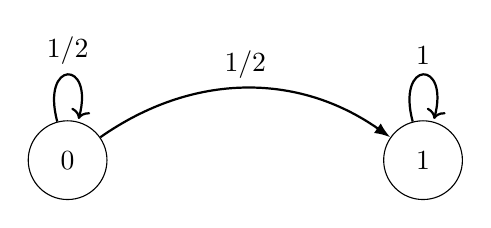
\begin{tikzpicture}[
  state/.style={circle, draw, minimum size=10mm},
  edge/.style={-{Latex[length=2mm]}, thick},
  bend angle=35
]
\node[state] (0) {$0$};
\node[state, right=35mm of 0] (1) {$1$};

\draw[edge] (0) edge[loop above] node {$1/2$} (0);
\draw[edge] (0) edge[bend left] node[above] {$1/2$} (1);
\draw[edge] (1) edge[loop above] node {$1$} (1);
\end{tikzpicture}
\end{center}

The transition matrix is
\[
P=
\begin{pmatrix}
\frac12 & \frac12\\
0 & 1
\end{pmatrix}.
\]

State $1$ is absorbing. From state $0$, there is a chance of moving to state $1$, and once the chain reaches state $1$, it can never return to state $0$.

\subsection{Using the Series Criterion for State 0}

Starting from state $0$, to be in state $0$ after $n$ steps, the chain must stay in state $0$ for all $n$ steps.

Each step has probability $1/2$ of staying in state $0$. Therefore,
\[
p_{00}^{(n)}=\left(\frac12\right)^n.
\]

Now calculate the series:
\[
\sum_{n=1}^{\infty}p_{00}^{(n)}
=
\sum_{n=1}^{\infty}\left(\frac12\right)^n.
\]

This is a geometric series:
\[
\sum_{n=1}^{\infty}\left(\frac12\right)^n
=
\frac{\frac12}{1-\frac12}
=1.
\]

Since
\[
\sum_{n=1}^{\infty}p_{00}^{(n)}=1<\infty,
\]
state $0$ is transient.

\subsection{Interpretation}

The expected number of future visits to state $0$ is finite. This makes sense from the diagram: eventually the chain may move to state $1$, and then it is trapped there forever.

\section{Example 2: A Recurrent State}

Consider the Markov chain with only one state:

\begin{center}
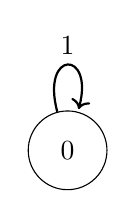
\begin{tikzpicture}[
  state/.style={circle, draw, minimum size=10mm},
  edge/.style={-{Latex[length=2mm]}, thick}
]
\node[state] (0) {$0$};
\draw[edge] (0) edge[loop above] node {$1$} (0);
\end{tikzpicture}
\end{center}

The transition matrix is
\[
P=(1).
\]

Starting from state $0$, the chain is always in state $0$. Therefore,
\[
p_{00}^{(n)}=1
\]
for every $n\geq 1$.

Now calculate the series:
\[
\sum_{n=1}^{\infty}p_{00}^{(n)}
=
\sum_{n=1}^{\infty}1.
\]

This sum diverges:
\[
\sum_{n=1}^{\infty}1=\infty.
\]

Therefore state $0$ is recurrent.

\subsection{Interpretation}

The chain returns to state $0$ at every time step. So the number of returns is infinite, and state $0$ is recurrent.

\section{Example 3: Recurrent Two-State Cycle}

Consider the Markov chain:

\begin{center}
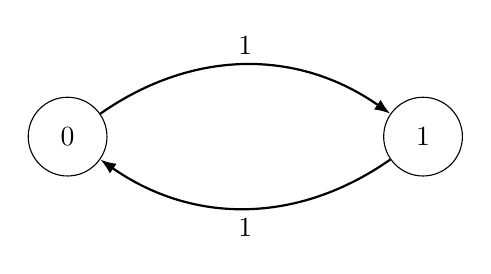
\begin{tikzpicture}[
  state/.style={circle, draw, minimum size=10mm},
  edge/.style={-{Latex[length=2mm]}, thick},
  bend angle=35
]
\node[state] (0) {$0$};
\node[state, right=35mm of 0] (1) {$1$};

\draw[edge] (0) edge[bend left] node[above] {$1$} (1);
\draw[edge] (1) edge[bend left] node[below] {$1$} (0);
\end{tikzpicture}
\end{center}

The transition matrix is
\[
P=
\begin{pmatrix}
0 & 1\\
1 & 0
\end{pmatrix}.
\]

Starting from state $0$:
\[
X_1=1,\quad X_2=0,\quad X_3=1,\quad X_4=0,\quad \ldots
\]

Thus,
\[
p_{00}^{(n)}
=
\begin{cases}
1, & n\text{ is even},\\
0, & n\text{ is odd}.
\end{cases}
\]

Then
\[
\sum_{n=1}^{\infty}p_{00}^{(n)}
=
0+1+0+1+0+1+\cdots.
\]

This sum diverges to infinity because there are infinitely many terms equal to 1.

Therefore state $0$ is recurrent. Similarly, state $1$ is recurrent.

\subsection{Important Note}

This chain is recurrent, but it is periodic. Recurrence and aperiodicity are different ideas.

\section{Example 4: A Transient State with Formula from Matrix Powers}

Consider
\[
P=
\begin{pmatrix}
a & 1-a\\
0 & 1
\end{pmatrix},
\qquad 0<a<1.
\]

The transition diagram is:

\begin{center}
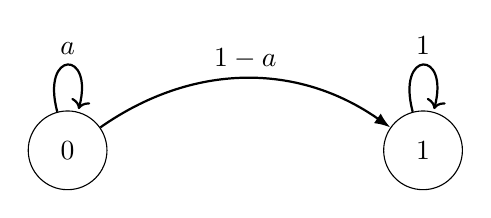
\begin{tikzpicture}[
  state/.style={circle, draw, minimum size=10mm},
  edge/.style={-{Latex[length=2mm]}, thick},
  bend angle=35
]
\node[state] (0) {$0$};
\node[state, right=35mm of 0] (1) {$1$};

\draw[edge] (0) edge[loop above] node {$a$} (0);
\draw[edge] (0) edge[bend left] node[above] {$1-a$} (1);
\draw[edge] (1) edge[loop above] node {$1$} (1);
\end{tikzpicture}
\end{center}

Starting from state $0$, to still be in state $0$ after $n$ steps, the chain must choose the self-loop $n$ times. Therefore,
\[
p_{00}^{(n)}=a^n.
\]

Then
\[
\sum_{n=1}^{\infty}p_{00}^{(n)}
=
\sum_{n=1}^{\infty}a^n
=
\frac{a}{1-a}.
\]

Since
\[
0<a<1,
\]
we have
\[
\frac{a}{1-a}<\infty.
\]

Therefore state $0$ is transient.

State $1$ is recurrent because it is absorbing.

\section{Practice Questions}

\begin{enumerate}[label=\textbf{Q\arabic*.}, leftmargin=1.2cm]
    \item Consider the chain
    \[
    P=
    \begin{pmatrix}
    \frac13 & \frac23\\
    0 & 1
    \end{pmatrix}.
    \]
    Use the series criterion to determine whether state $0$ is recurrent or transient.

    \item Consider the chain
    \[
    P=
    \begin{pmatrix}
    1 & 0\\
    0.4 & 0.6
    \end{pmatrix}.
    \]
    Use the series criterion to determine whether state $1$ is recurrent or transient.

    \item Consider the deterministic cycle
    \[
    0\to 1,\qquad 1\to 2,\qquad 2\to 0.
    \]
    Find $p_{00}^{(n)}$ and use the series criterion to classify state $0$.

    \item Suppose that for a Markov chain,
    \[
    p_{ii}^{(n)}=\left(\frac34\right)^n.
    \]
    Is state $i$ recurrent or transient?

    \item Suppose that for a Markov chain,
    \[
    p_{ii}^{(n)}=\frac{1}{n}.
    \]
    Based on the series criterion, is state $i$ recurrent or transient?

    \item Suppose that for a Markov chain,
    \[
    p_{ii}^{(n)}=\frac{1}{n^2}.
    \]
    Based on the series criterion, is state $i$ recurrent or transient?

    \item Explain in words why a finite value of
    \[
    \sum_{n=1}^{\infty}p_{ii}^{(n)}
    \]
    means state $i$ is transient.

    \item Explain in words why an infinite value of
    \[
    \sum_{n=1}^{\infty}p_{ii}^{(n)}
    \]
    means state $i$ is recurrent.
\end{enumerate}

\section{Answers}

\subsection*{Answer 1}

The transition matrix is
\[
P=
\begin{pmatrix}
\frac13 & \frac23\\
0 & 1
\end{pmatrix}.
\]

Starting from state $0$, to be in state $0$ after $n$ steps, the chain must stay in state $0$ for all $n$ steps. Each self-loop has probability $1/3$.

Therefore,
\[
p_{00}^{(n)}=\left(\frac13\right)^n.
\]

Then
\[
\sum_{n=1}^{\infty}p_{00}^{(n)}
=
\sum_{n=1}^{\infty}\left(\frac13\right)^n.
\]

This is a geometric series:
\[
\sum_{n=1}^{\infty}\left(\frac13\right)^n
=
\frac{\frac13}{1-\frac13}
=
\frac12.
\]

Since the sum is finite, state $0$ is transient.

\[
\boxed{\text{State }0\text{ is transient.}}
\]

\subsection*{Answer 2}

The transition matrix is
\[
P=
\begin{pmatrix}
1 & 0\\
0.4 & 0.6
\end{pmatrix}.
\]

Starting from state $1$, to be in state $1$ after $n$ steps, the chain must stay in state $1$ for all $n$ steps. Each self-loop has probability $0.6$.

Therefore,
\[
p_{11}^{(n)}=(0.6)^n.
\]

Then
\[
\sum_{n=1}^{\infty}p_{11}^{(n)}
=
\sum_{n=1}^{\infty}(0.6)^n.
\]

This is a geometric series:
\[
\sum_{n=1}^{\infty}(0.6)^n
=
\frac{0.6}{1-0.6}
=
1.5.
\]

Since the sum is finite, state $1$ is transient.

\[
\boxed{\text{State }1\text{ is transient.}}
\]

State $0$ is absorbing and recurrent, but the question asked about state $1$.

\subsection*{Answer 3}

The chain is
\[
0\to 1,\qquad 1\to 2,\qquad 2\to 0.
\]

Starting from state $0$, the chain returns to state $0$ after 3 steps, 6 steps, 9 steps, and so on.

Therefore,
\[
p_{00}^{(n)}
=
\begin{cases}
1, & n=3,6,9,\ldots,\\
0, & \text{otherwise}.
\end{cases}
\]

Then
\[
\sum_{n=1}^{\infty}p_{00}^{(n)}
=
0+0+1+0+0+1+0+0+1+\cdots.
\]

This sum diverges because there are infinitely many terms equal to 1.

Therefore state $0$ is recurrent.

\[
\boxed{\text{State }0\text{ is recurrent.}}
\]

\subsection*{Answer 4}

We are given
\[
p_{ii}^{(n)}=\left(\frac34\right)^n.
\]

Then
\[
\sum_{n=1}^{\infty}p_{ii}^{(n)}
=
\sum_{n=1}^{\infty}\left(\frac34\right)^n.
\]

This is a geometric series with ratio $3/4$, so
\[
\sum_{n=1}^{\infty}\left(\frac34\right)^n
=
\frac{\frac34}{1-\frac34}
=3.
\]

Since the sum is finite, state $i$ is transient.

\[
\boxed{\text{State }i\text{ is transient.}}
\]

\subsection*{Answer 5}

We are given
\[
p_{ii}^{(n)}=\frac1n.
\]

Then
\[
\sum_{n=1}^{\infty}p_{ii}^{(n)}
=
\sum_{n=1}^{\infty}\frac1n.
\]

This is the harmonic series, and it diverges:
\[
\sum_{n=1}^{\infty}\frac1n=\infty.
\]

Therefore state $i$ is recurrent.

\[
\boxed{\text{State }i\text{ is recurrent.}}
\]

\subsection*{Answer 6}

We are given
\[
p_{ii}^{(n)}=\frac1{n^2}.
\]

Then
\[
\sum_{n=1}^{\infty}p_{ii}^{(n)}
=
\sum_{n=1}^{\infty}\frac1{n^2}.
\]

The series
\[
\sum_{n=1}^{\infty}\frac1{n^2}
\]
converges. Therefore,
\[
\sum_{n=1}^{\infty}p_{ii}^{(n)}<\infty.
\]

Hence state $i$ is transient.

\[
\boxed{\text{State }i\text{ is transient.}}
\]

\subsection*{Answer 7}

The sum
\[
\sum_{n=1}^{\infty}p_{ii}^{(n)}
\]
is the expected total number of returns to state $i$.

If this sum is finite, then the chain is expected to return to state $i$ only a finite number of times. This means there is a positive probability that after leaving state $i$, the chain never comes back.

Therefore state $i$ is transient.

\subsection*{Answer 8}

The sum
\[
\sum_{n=1}^{\infty}p_{ii}^{(n)}
\]
is the expected total number of returns to state $i$.

If this sum is infinite, then the chain is expected to return to state $i$ infinitely often. This means that starting from state $i$, the chain returns to $i$ eventually with probability 1.

Therefore state $i$ is recurrent.

\end{document}
